\section {Stavba pulzního oxymetru}
\subsection {Volba platformy}
Jednou z hlavních priorit při designování našeho oxymetru bylo, aby ho bylo možné jednoduše používat připevněný na jednom prstu. Hlavní prioritou tedy bylo, aby byl co nejmenší a nejlehčí. První možností, kterou jsme identifikovali bylo Arduino Micro a desky postavené na jeho designu.
\par Arduino Micro je jednodeskový mikroprocesor od společnosti Arduino, který se zaměřuje na to, aby byl co nejmenší. Díky tomu, že design desek je zveřejněn pod licencí Creative Commons, tak může kdokoli desky upravit a svoji verzi prodávat. To nám umožnilo si najít Arduino Micro upravené tak, aby neobsahovalo věci, které jsme neplánovali používat a díky tomu bylo ještě menší a levnější.
\par Tato možnost ale měla i své problémy. Hlavním z těchto problémů bylo napájení. První možností, jak desku napájet je její USB Micro-B konektor, který vyžaduje stabilních 5 V. Tento port umožňuje při testování a u některých projektů desku jednoduše napájet, a to buď ze zásuvky s adaptérem, anebo z většiny přenosných akumulátorů, které obsahují potřebné stejnosměrné měniče napětí a USB porty. Toto řešení ale nebylo vhodné pro naše použití, protože výsledný oxymetr musel být přenosný a i zmíněné přenosné akumulátory byly moc velké a těžké. Druhou možností, jak desku napájet je napájecí pin na který stačí přivést 7–12 V a deska si sama toto napětí převede na potřebných 5 V. Tato možnost ale také nebyla zcela ideální, protože většina baterií a akumulátorů které by bylo možné v oxymetru použít měly o dost nižší napětí, což by znamenalo, že bychom museli použít více těchto zdrojů energie v sérii za sebou. To by nejen udělalo zdroj energie moc těžký a velký pro naše použití, ale zároveň by to v případě akumulátorů udělalo nejen nabíjení o dost složitější. Z těchto důvodů jsme se vydali hledat jinou, a pro náš projekt použitelnější, platformu.
\par 21. ledna 2021 vydala Raspberry Pi Foundation svůj první jednodeskový mikroprocesor, který se jmenuje Raspberry Pi Pico. Tento mikroprocesor nás zaujal hned z několika důvodů. Hlavním z nich je, jakým způsobem u něj funguje napájení. Pi Pico má vestavěný spínaný zdroj typu buck-boost, který dokáže vytvořit potřených 3,3 V ze širokého rozsahu vstupních napětí (1,8–5,5 V). Toto bylo pro naše použití ideální, a to nejen proto, že jsme si mohli vybrat baterii podle naší potřeby, ale i proto, že má vysokou efektivitu při převodu energie, což umožnilo delší provoz bez nabíjení. Další z velkých výhod je, že Pi Pico je podobně cenově dostupné jako výše zmíněné adaptace designů společnosti Arduino. V České republice je v době psaní této práce dostupné za 109 Kč. Další výhodou je dobrá dokumentace, a to nejen pro samotný procesor \citep{rp2040DS}, jak bývá zvykem u zařízení kde většina funkcionality je určena hlavním čipem, který je dobře zdokumentován, ale i přímo pro celé Pi Pico \citep{picoDS}, která nejen zajišťuje, že jsou jednoduše dostupné informace o obvodech okolo samotného procesoru, ale také radí co a jak dělat při práci s Picem. Tyto dvě dokumentace se v průběhu projektu ukázaly jako velmi užitečné. Jedinou nevýhodou byla znatelně větší velikost, která ale byla vyvážena tím, jak flexibilní pro nás byl systém pro napájení. Nakonec jsme se tedy rozhodli používat Raspberry Pi Pico.
\subsection {Prototypy}
\subsubsection {První prototypy}
\begin{figure}[ht]
  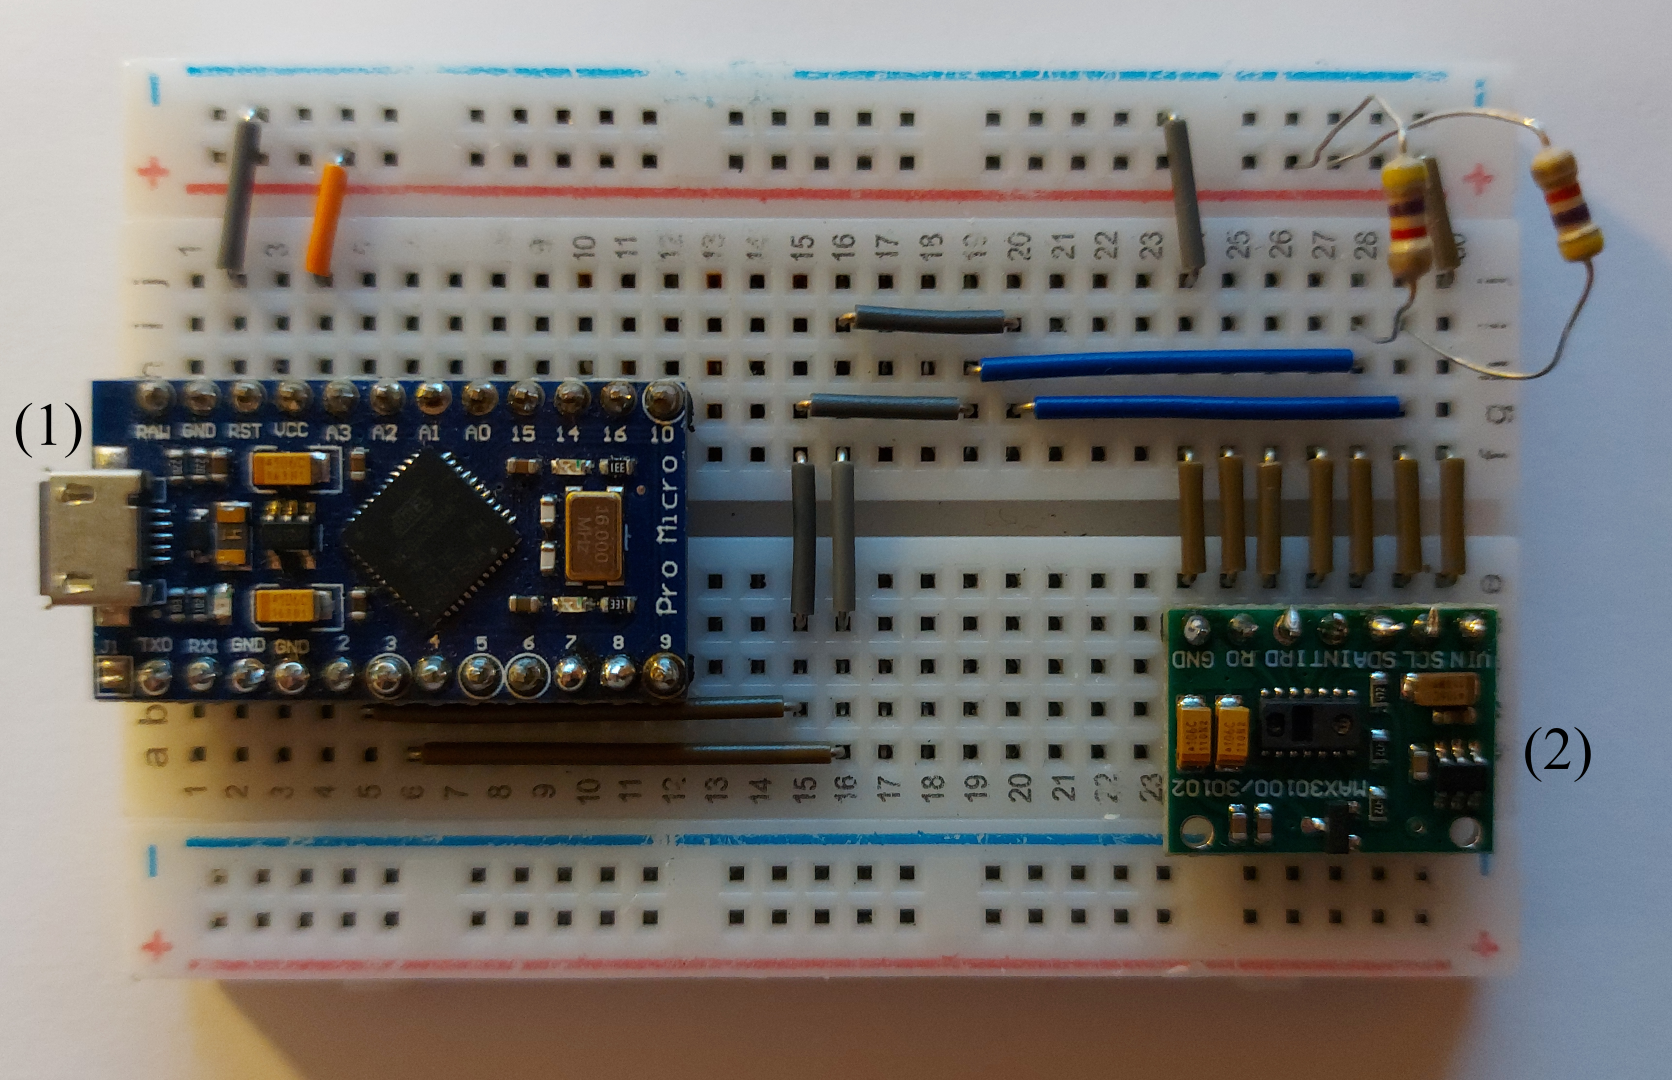
\includegraphics[scale=0.27, center]{Kapitoly/Prakticka/Obrazky/První_prototypy.png}
  \caption [První prototyp]{Takto vypadaly první prototypy. (1) je jednodeskový mikroprocesor a (2) je oxymetr. Vlastní dílo}
  \label{fig:První_prototyp}
\end{figure}
Nejjednodušší způsob, jak udělat první prototyp je ke všemu připájet piny a začít stavět na nepájivém poli. To jsme také udělali s naším prvním prototypem, který můžete vidět na obrázku \ref{fig:První_prototyp}. V této fázi bylo hlavní zjišťovat vhodnost jednotlivých součástek pro naše využití a vyzkoušet, zda fungují.
\paragraph{MAX30100}
Jako samotný oxymetr jsme se rozhodli použít MAX30100, který je jedním z nejčastějších a zároveň jednoduše sehnatelných oxymetrů na trhu. \citep{max30100}. Plošný spoj na kterém se MAX30100 nachází již obsahuje všechny důležité podpůrné komponenty: převodník na 3,3 V, další převodník na 1,8 V (obě napěťové hladiny jsou nutností pro operaci MAX30100) a další pasivní komponenty. Jednou ze zajímavých vlastností designu těchto desek jsou i pullup rezistory. Tyto rezistory jsou na $I^2C$ sběrnici a propojují ji s 1,8 V. Toto není zcela obvyklý design, protože myšlenkou této sběrnice je, že zařízení tyto rezistory nemají, a že samotná sběrnice zařídí, aby se tyto rezistory v ní právě jednou nacházeli. Toto ale začíná být problém, až pokud je na jedné sběrnici více takovýchto zařízení. Větším problémem je, že tyto pullup rezistory vedou na 1,8 V, a ne na napětí, které využívají ostatní připojená zařízení. Toto není žádný problém, pokud všechna zařízení komunikují na 1,8 V, ale je zcela zbytečné pro Arduino, které komunikuje na 5 V. 1,8 V je dle našeho testování funkční u 3,3V zařízení, ale ani v tomto případě není doporučitelné, protože nemusí být spolehlivé. Proto je většinou potřeba připojit své 4,7kΩ pullupové rezistory. Rezistory na oxymetru je také možné odpájet, ale vzhledem k tomu, že jsou tak velké a jen na 1,8 V, ve skutečnosti nespotřebovávají tolik energie, aby byl velký problém je tam na oxymetru nechat.
\subsubsection {Druhý prototyp}
Druhý prototyp měl za úkol jednak vyřešit problémy které dělalo okolní světlo oxymetru při měření, a také postavit takový prototyp, který by byl více reprezentativním testem pro finální verzi.
\begin{figure}[ht]
  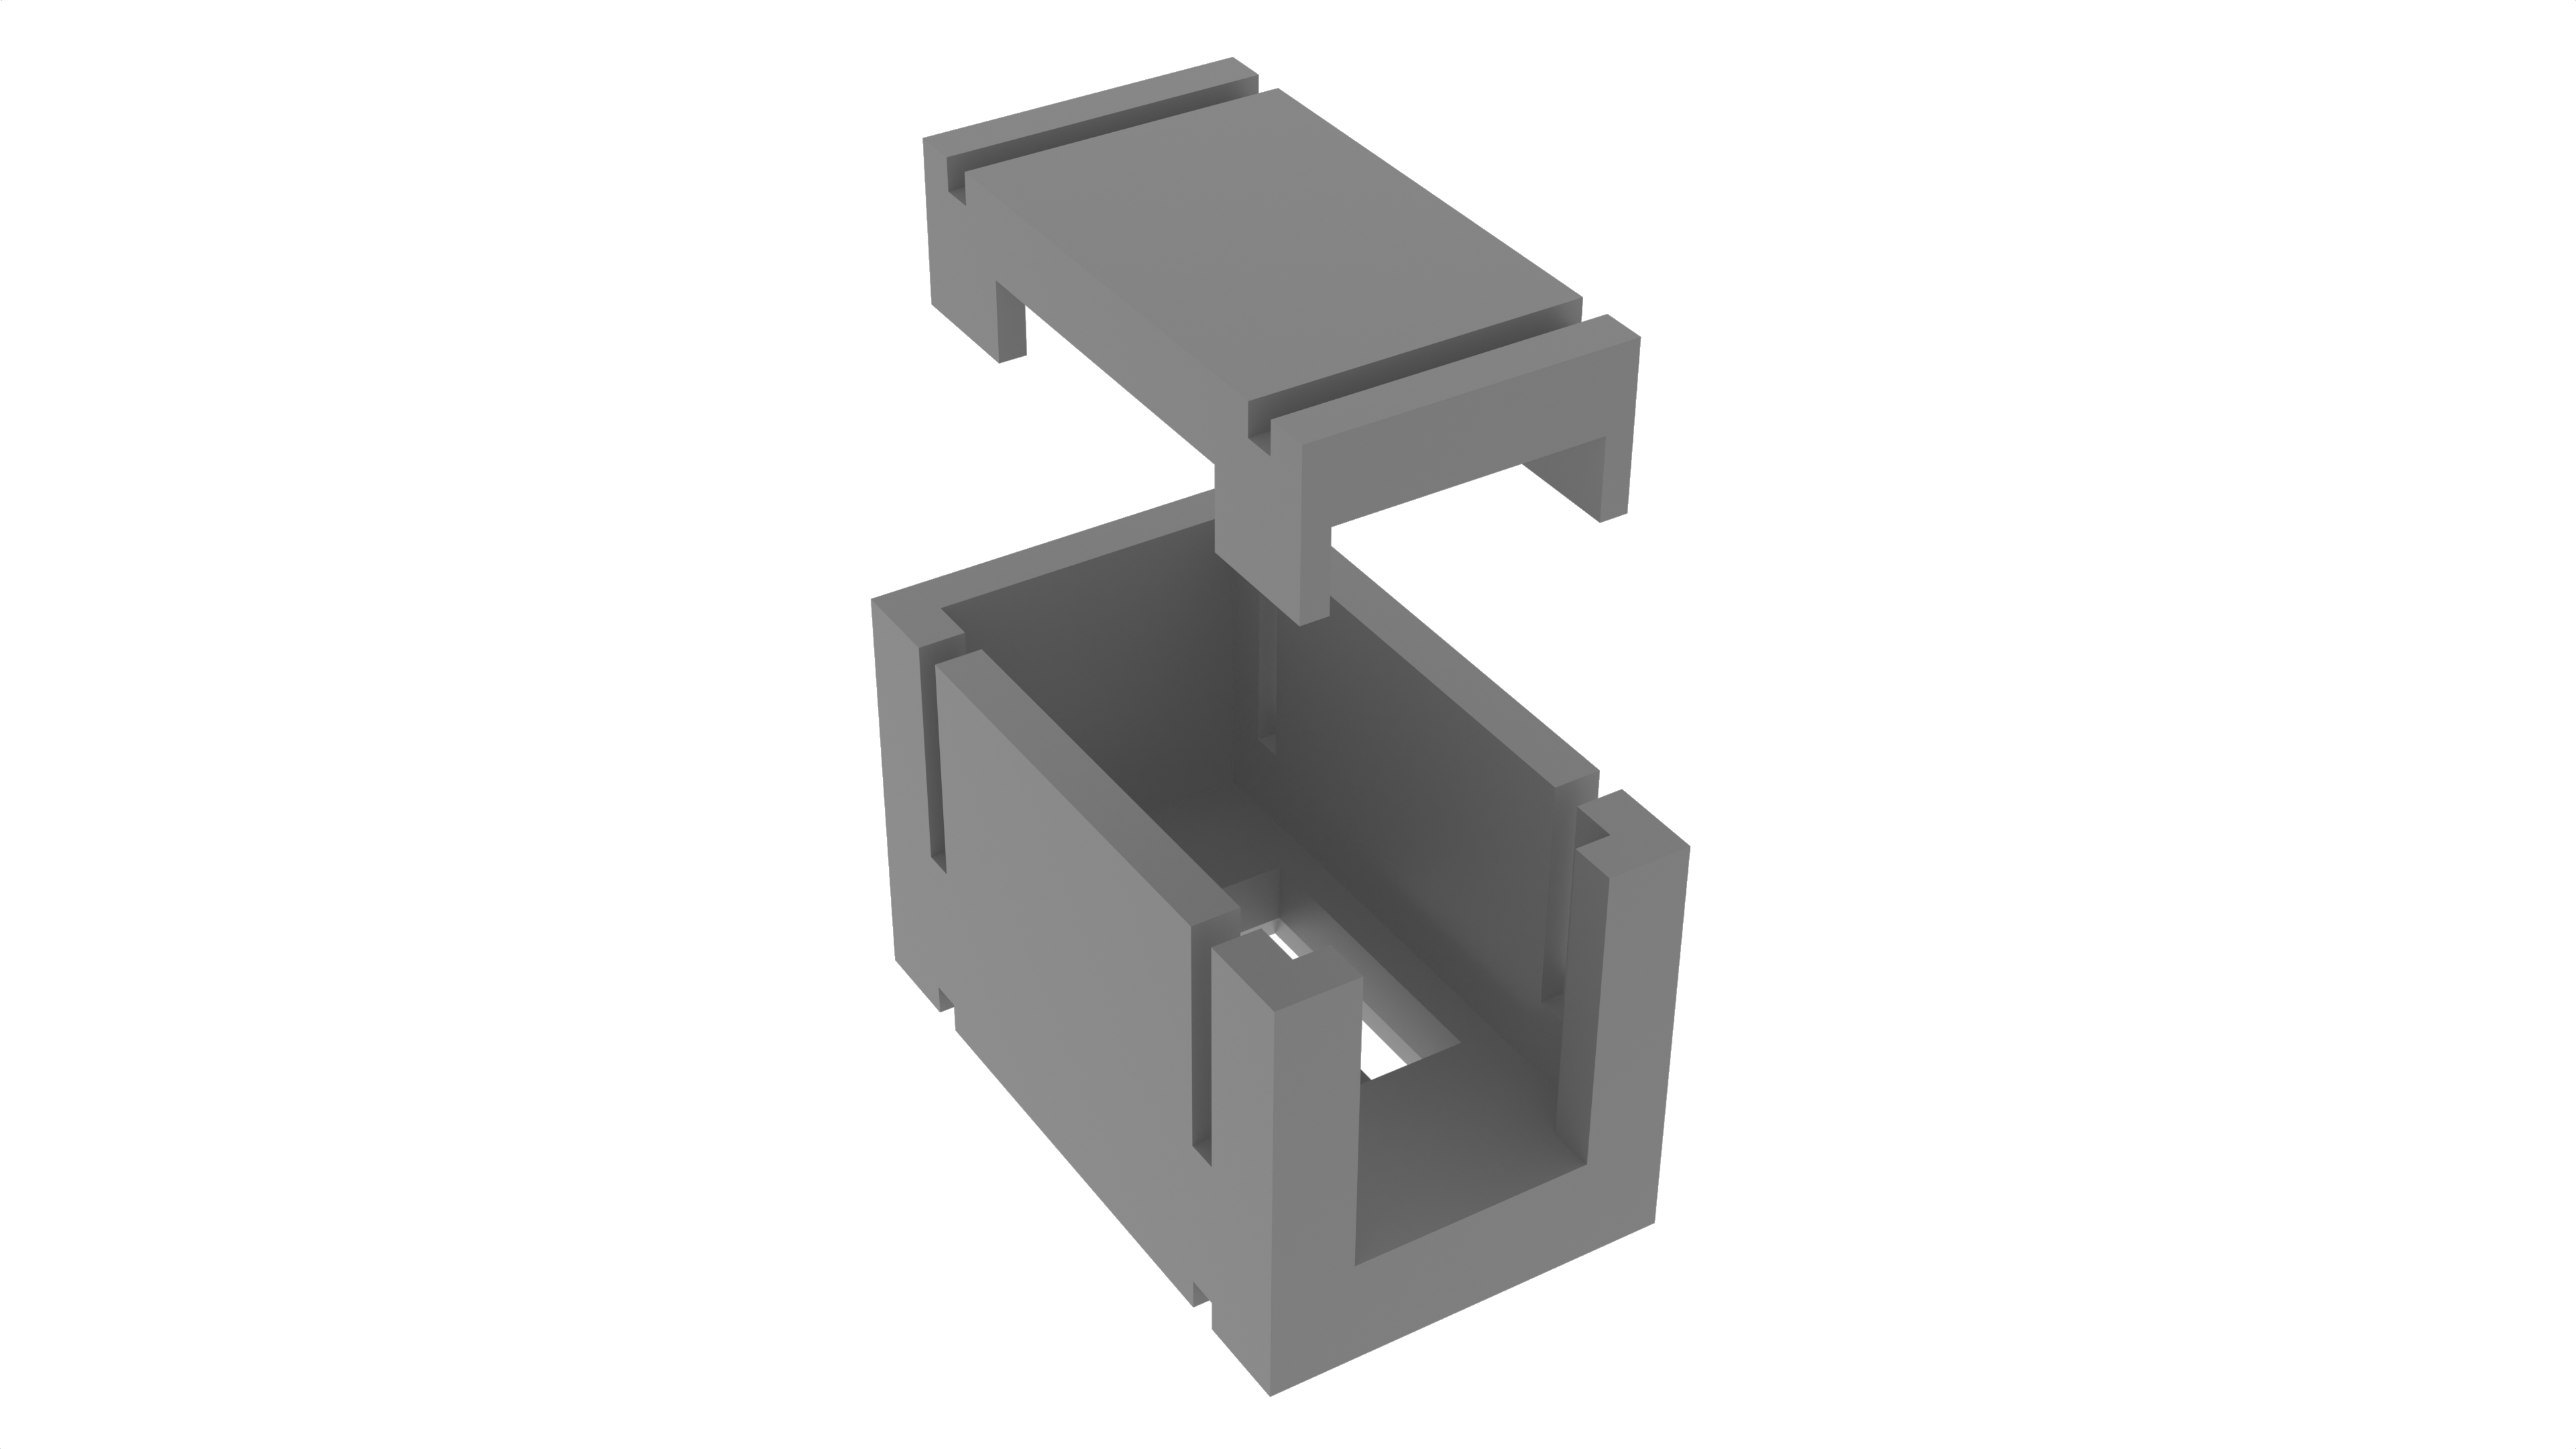
\includegraphics[scale=0.13, center]{Kapitoly/Prakticka/Obrazky/Druhý_prototyp2_w.png}
  \caption [3D model druhého prototypu]{První 3D tištěný prototyp. Skládá se jen ze dvou částí - spodní komory pro prst, jež obsahovala i místo pro oxymetr a horní části mající za úkol pomocí gumičky komoru seshora i s prstem uzavřít. Vlastní dílo}
  \label{fig:3D_model_druhého_prototypu}
\end{figure}
\paragraph{3D tisk / modelování}
Tento první model se nakonec skládal jen ze dvou částí: spodní komory pro prst obsahující i místo pro oxymetr a horní co měla za úkol pomocí gumičky komoru ze shora i s prstem uzavřít. Tento design se ukázal býti efektivním a zajistil spolehlivé měření. Tento design je převážně dílem Benjamina Swarta a pomohl nám při modelování všech ostatních modelů, které jsou naši úpravou tohoto modelu.
\subsubsection {Finální verze}
Po úspěchu druhého prototypu byl čas pracovat na prototypu, který již spojuje vše dohromady, a má zespoda velkou část, ve které se schovají všechny obvody.
\begin{figure}[ht]
  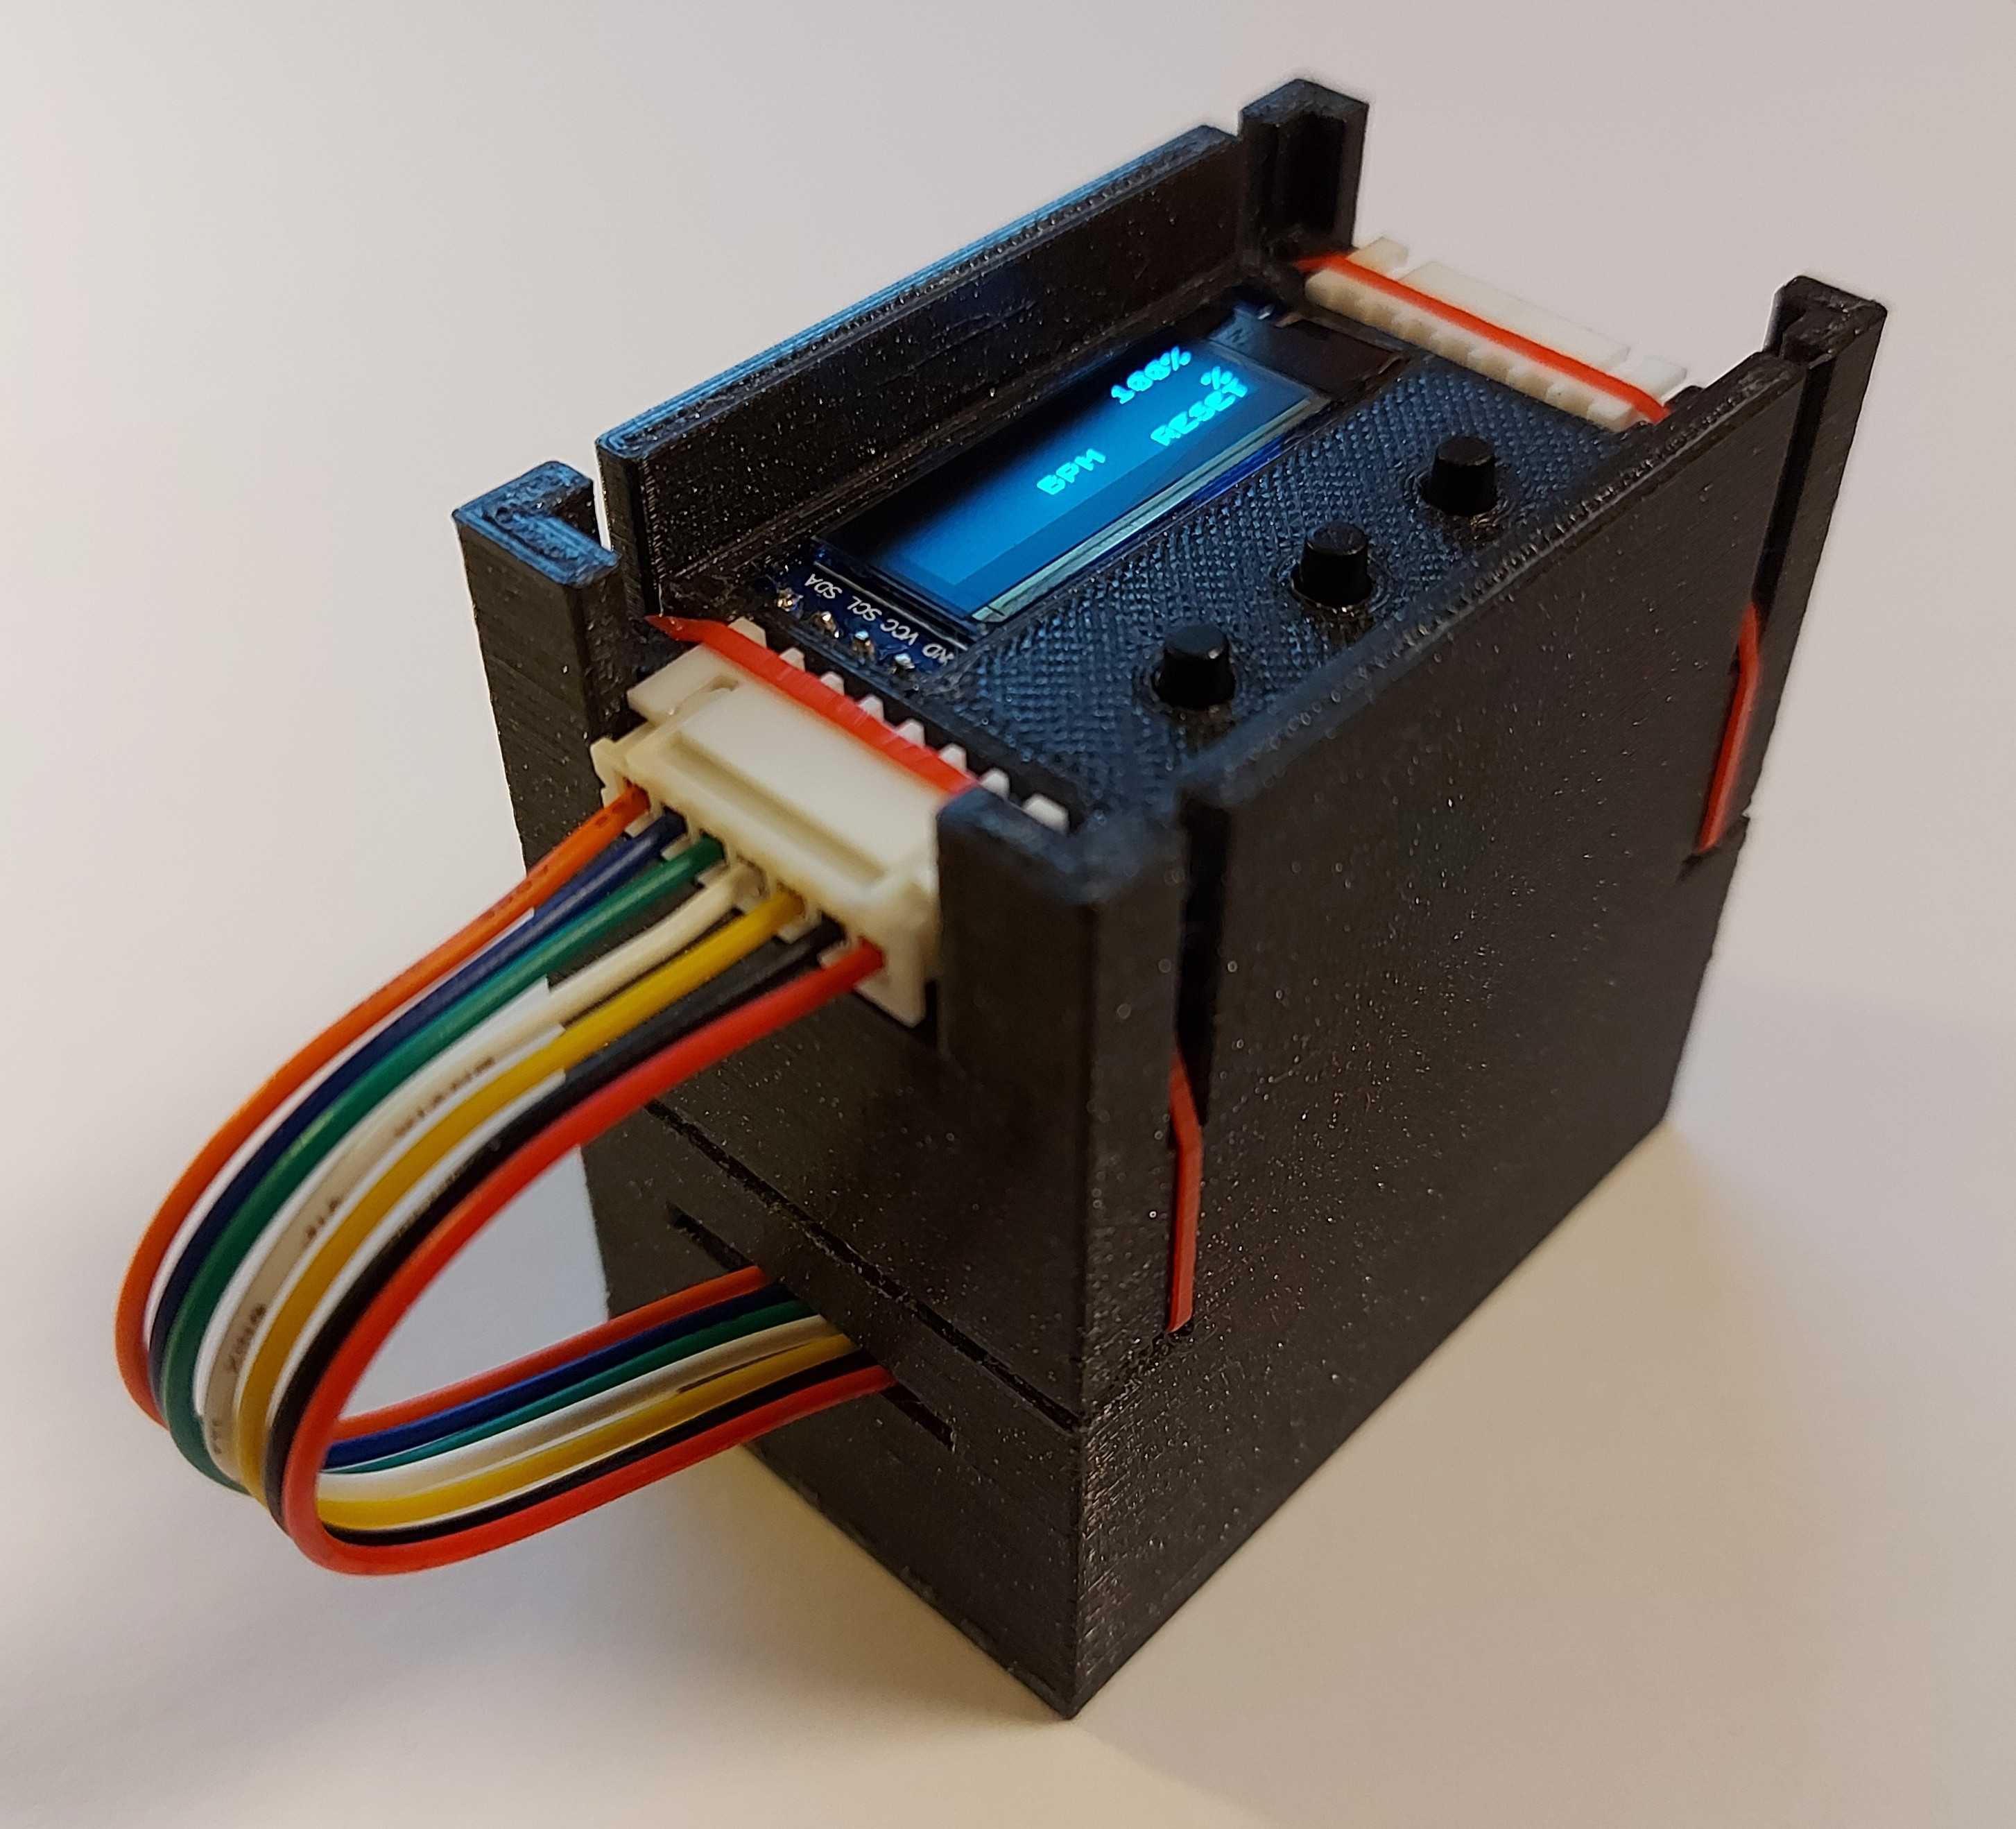
\includegraphics[scale=0.12, center]{Kapitoly/Prakticka/Obrazky/Finální_prototyp.jpg}
  \caption [Finální prototyp]{Hotový pulzní oxymetr v pohledu zprava zezadu. Vlastní dílo}
  \label{fig:Finální_prototyp}
\end{figure}
\begin{figure}[ht]
  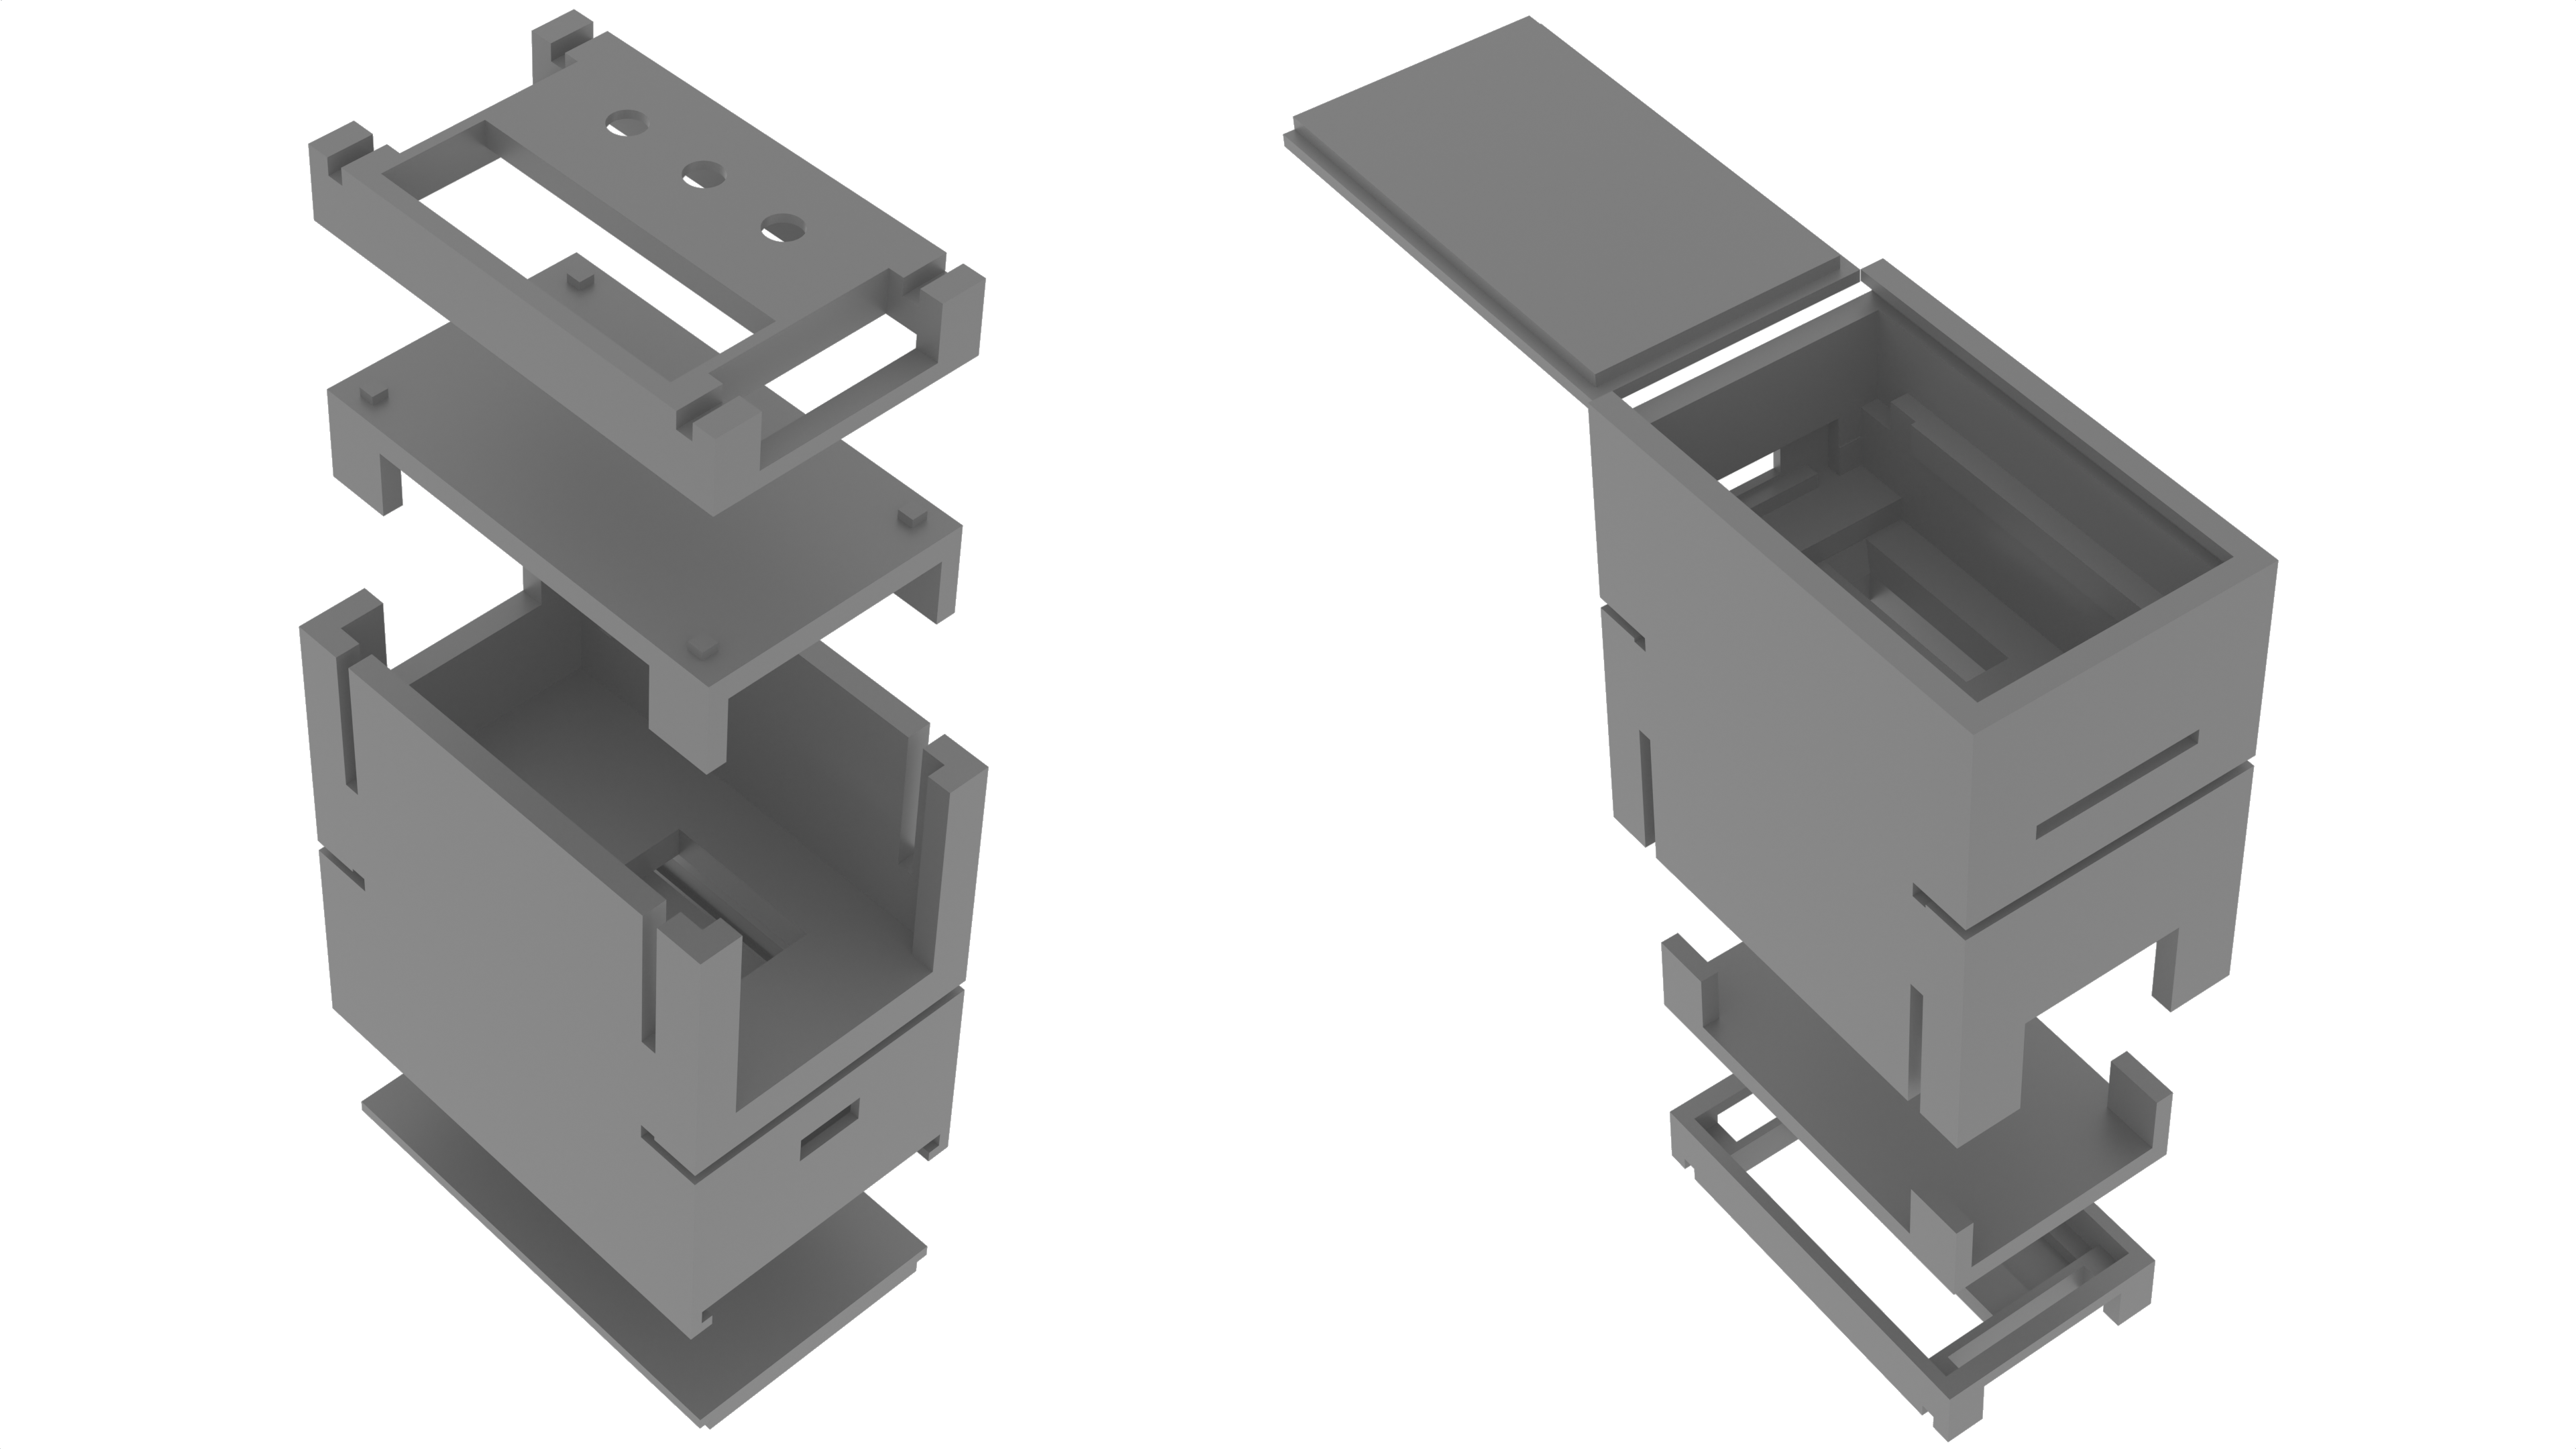
\includegraphics[scale=0.13, center]{Kapitoly/Prakticka/Obrazky/Finální.png}
  \caption [3D model finálního prototypu]{3D model finálního prototypu, který již obsahuje  všechny potřebné kusy i s místy na elektroniku a dírami na displej a tlačítka. Vlastní dílo}
  \label{fig:3D_model_finálního_prototypu}
\end{figure}
\paragraph{Nový model}
Design tohoto prototypu začal pečlivým měřením všech součástek a stavěním samotného 3D modelu. Při tomto procesu bylo velmi důležité dát si pozor, aby všude byly dostatečné rezervy.
\paragraph{Displej a tlačítka}
Zajímavým problémem bylo i umístnění displeje a ovládacích tlačítek. Náš oxymetr bohužel nemá šikovnou přístupnou stranu, kam by se tyto věci vešly. Jedním z jediných jednoduchých řešení by mohlo být dát displej z boku samotného oxymetru. Toto řešení by ale bylo nejspíš docela problematické při používání zařízení. Jedním z důvodů je obecná nešikovnost místa, vzhledem k tomu že na tom místě budou pravděpodobně překážet prsty. Navíc by v tuto chvíli potřebné naklánění oxymetru a tlačení na něj ze strany mohlo ovlivnit měření dat. Druhým z důvodů je to, že pokud je displej na jedné straně oxymetru, je relativně pohodlné ovládání na jedné z rukou, avšak by bylo náročné používat ho na té druhé, a to jednoduše proto, že by displej mířil pryč od samotného uživatele. Řešení, které jsme nakonec použili je displej a tlačítka vestavět do samotné horní posuvné části oxymetru a propojit se zbytkem kabely vedenými zvenku. Tyto kabely mohou být odpojeny a připojeny z druhé strany modulu pro používání na druhé ruce. Toto řešení se ukázalo býti docela elegantním a mělo jedinou malou nevýhodu, a to tu, že to udělalo celý oxymetr větším. To se stalo proto, že kromě sxamotného dispeje, který má nějakou velikost, musí být kolem něj trochu plastu pro udržení struktury, a na obou koncích musí být konektory pro zmíněný propojovací kabel. Tato prostorová limitace ale také znamenala zvětšení prostoru na práci v těle samotného oxymetru. Konkrétně se nám díky tomuto nucenému zvětšení vešel do spodní části větší, 900mAh akumulátor.
\begin{figure}[ht]
    \def\svgwidth{\columnwidth}
    \input{Kapitoly/Prakticka/Obrazky/oxymetr.pdf_tex}
    \caption [Schematický diagram obvodu]{Schematický diagram celého obvodu. U1 je samotné Raspberry Pi Pico. Jeho $I^2C$ sběrnice má na sobě 4,7k pullupové rezistory. Tato sběrnice je také rovnou připojena k oxymetru (U3), ale také pomocí sedmipinového konektoru J3 přímo k modulu s displejem. Modul s displejem také obsahuje 3 talčítka, z nichž 2 již mají připojeny 10kΩ pulldownové rezistory. Na straně Pica jsou tato tlačítka propojena s GPIO10 a GPIO11 a tlačítko bez rezistoru je připojeno k pinu RUN. K Picu je také připojen akumulátor, a to skrz jeho nabíjecí a ochraný modul a Schottkyho diodu. Vlastní dílo}
    \label{fig:Diagram}
\end{figure}
\subsection {Software}
Nedílnou součástí našeho oxymetru je i jeho software. Hlavní dvě věci, které musí software dělat je komunikovat s našimi dvěma $I^2C$ zařízeními. Toto se děje po jedné $I^2C$ sběrnici a je převážně zařizováno knihovnami určenými pro daná zařízení. Pro oxymetr jsem použili knihovnu MAX30100lib, která nejen zařizuje komunikaci, ale také přímo počítá tep a $SpO_2$. Druhým takto připojeným zařízením je displej. Pro komunikaci s ním jsme využili knihovny U8g2. Ta nám dovolila jednoduše psát potřebný text na jakoukoli část displeje. Poslední z komponent určených pro  uživatele jsou tlačítka. Jedno z nich je již připojeno mezi pinem RUN a GND, což znamená, že je-li tlačítko zmáčknuté, procesor neběží. To pro uživatele znamená, že se Pi Pico restartuje. Toto tlačítko je tedy vyřešeno přes hardware a nemusíme ho v software řešit. Zbylá dvě tlačítka jsou připojena k pinům GPIO10 a GPIO11 a mají 10kΩ pullup rezistor. Je tedy možné je použít jako vstupní periferii dle libosti. Další důležitou funkcí je část kódu, která pomocí měření vstupního napětí z akumulátoru říká kolik v něm ještě zbývá energie, nebo, v případě že je Pi Pico zrovna připojené k externímu zdroji, o tom podává informaci. Poslední skrytou funkcí je možnost zaznamenávat (a následně z počítače stáhnout) naměřená data. Data se zaznamenávají automaticky od zapnutí do velkého seznamu. Po připojení k počítači je poté možné sériovou linkou poslat příkaz „D“, který když Pi Pico dostane, vypíše všechna data, která zatím naměřilo. Tohoto lze dosáhnout automaticky pomocí programu v Pythonu (příloha \ref{appn:Python}), který z takto získaných dat automaticky vytvoří CSV soubor.